\documentclass[11pt,a4paper]{article}

\usepackage[utf8]{inputenc}
\usepackage[T1]{fontenc}
\usepackage[margin=2.4cm]{geometry}
\usepackage{amsmath,amssymb}
\usepackage{graphicx}
\usepackage{booktabs}
\usepackage{caption}
\usepackage{subcaption}
\usepackage{xcolor}
\usepackage{hyperref}
\usepackage[protrusion=true,expansion=false]{microtype}
\usepackage{enumitem}
\usepackage{titlesec}

\hypersetup{colorlinks=true,linkcolor=black!70!blue,urlcolor=blue!60!black}

\titleformat{\section}{\large\bfseries}{\thesection.}{0.6em}{}
\titleformat{\subsection}{\normalsize\bfseries}{\thesubsection}{0.5em}{}
\titlespacing*{\section}{0pt}{1.0em}{0.4em}
\titlespacing*{\subsection}{0pt}{0.7em}{0.2em}

\setlength{\parindent}{0pt}
\setlength{\parskip}{0.4em}
\captionsetup{font=small,labelfont=bf,skip=4pt}

\title{\vspace{-1.5em}\textbf{Scenario Analysis: MBS Prepayment under\\
Interest Rate Shocks}\\[0.3em]
\large IR\&C Assignment 3, Part E(iv) --- Spring 2026}
\author{Yueqi Lin\\\small MTH 9877, Baruch College}
\date{May 2026}

\begin{document}
\maketitle
\vspace{-1.2em}

% =================================================================
\section{Introduction}
% =================================================================

Mortgage prepayment is driven by the rate incentive $\rho_t = r_{\text{orig}} - r_{\text{market}}(t)$:
when market rates fall, borrowers can reduce their monthly payment by refinancing, and the
prepayment hazard rises. This optionality embeds negative convexity in mortgage-backed
securities (MBS): as rates fall, prepayments return principal at par, capping price
appreciation. Quantifying this sensitivity is the core task of MBS risk management.

This section stress-tests prepayment models by shocking market rates by $\pm 100$, $\pm 200$,
and $\pm 300$\,bp and tracing the response through five analyses:
shock sensitivity, survival curves, the prepayment S-curve, 2D interaction surfaces,
and a Monte Carlo MBS cash flow projection.

% =================================================================
\section{Model Setup}
% =================================================================

\textbf{Primary model}: the Andersen--Gill TV Cox from E(ii), fitted on 500K loan-month rows
(vintage $\le 2016$). \texttt{rate\_incentive} is a direct time-varying covariate, so a
market rate shock of $\Delta r$\,bp shifts the incentive by $-\Delta r/100$\,pp, producing
an analytic hazard response:
\begin{equation}
    \Delta\log h(t) = \hat\beta_{\text{ri}} \times \frac{-\Delta r}{100},
    \quad \hat\beta_{\text{ri}} = 0.041 \text{ (HR} = 1.042 \text{ per 100\,bp)}.
\end{equation}

The calibrated baseline hazard $\hat{H}_0(t)$ gives survival curves with realistic
10-year survival probabilities and CPR figures, making WAL and price calculations
economically meaningful.

\textbf{Contrast model}: partner's DeepCox from Part D (68 origination features, no market-rate
channel). Rate shocks must be applied to \texttt{OriginalInterestRate} as a \emph{counterfactual},
illustrating the fundamental limitation of static models for scenario analysis.

\textbf{Representative loan}: \$300K UPB, 6.5\% coupon, baseline market rate 7.0\%.

% =================================================================
\section{Rate Shock Sensitivity}
% =================================================================

\begin{figure}[h]
    \centering
    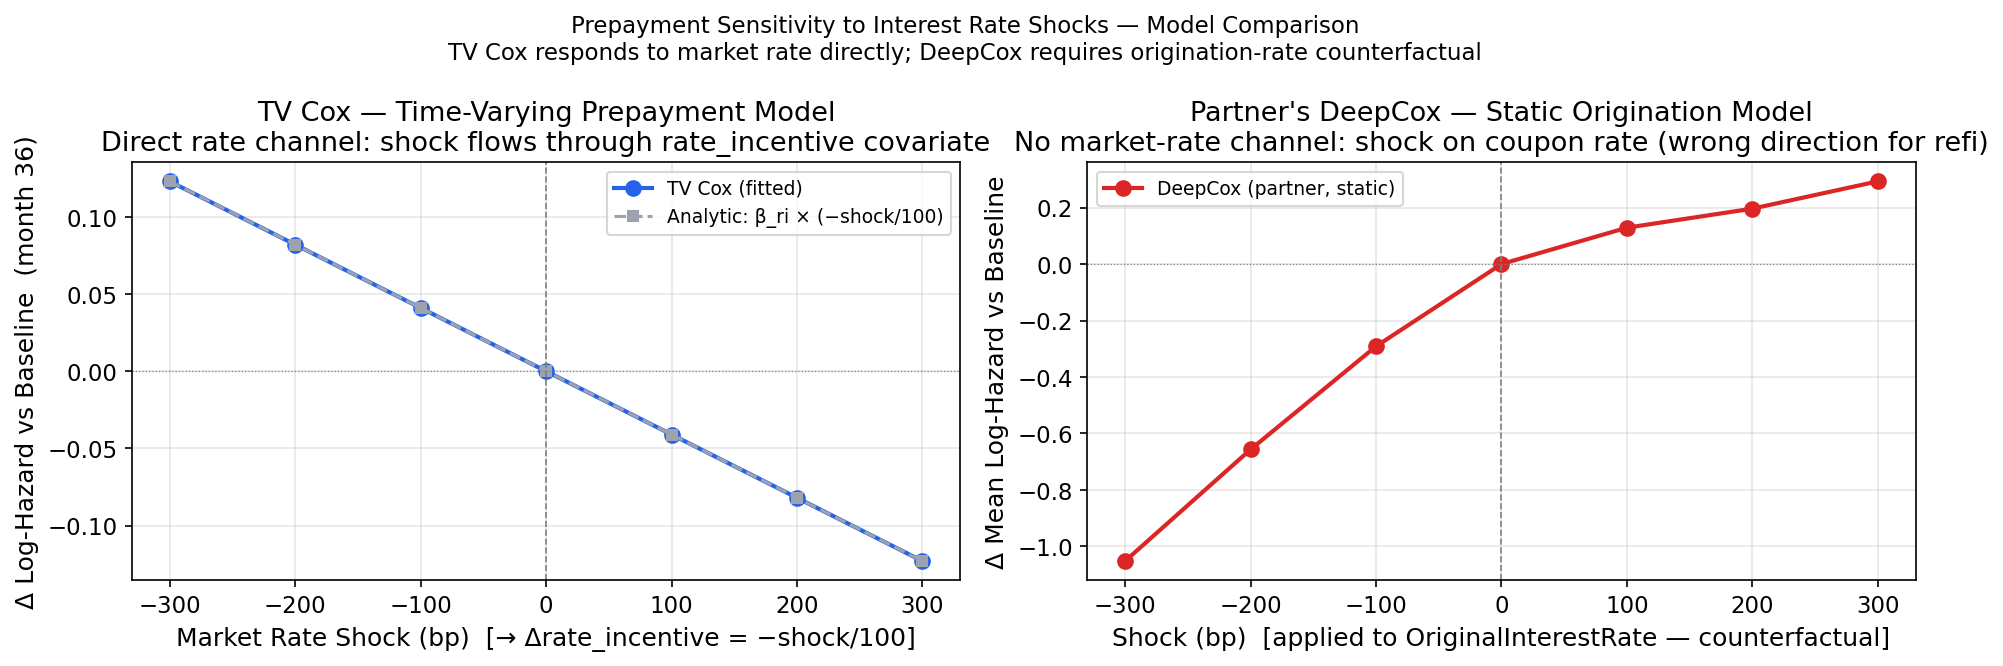
\includegraphics[width=\linewidth]{processed/Eiv_shock_comparison}
    \caption{$\Delta\log h$ vs.\ baseline at month 36 under seven rate scenarios.
      Left: TV Cox (blue dots) overlaps the analytic formula (grey dashes) exactly.
      Right: DeepCox produces the opposite sign --- a 300\,bp rate cut lowers
      the predicted hazard by 1.05, because the model interprets a lower
      \texttt{OriginalInterestRate} as less refinancing incentive relative to coupon.}
\end{figure}

\begin{center}
\small
\begin{tabular}{lrrr}
\toprule
\textbf{Shock} & \textbf{TV Cox $\Delta\log h$} & \textbf{Analytic} & \textbf{DeepCox $\Delta\log h$} \\
\midrule
$-300$\,bp & $+0.123$ & $+0.123$ & $-1.052$ \\
$-200$\,bp & $+0.082$ & $+0.082$ & $-0.657$ \\
$-100$\,bp & $+0.041$ & $+0.041$ & $-0.291$ \\
Baseline   &  $0.000$ &  $0.000$ &  $0.000$ \\
$+100$\,bp & $-0.041$ & $-0.041$ & $+0.129$ \\
$+200$\,bp & $-0.082$ & $-0.082$ & $+0.196$ \\
$+300$\,bp & $-0.123$ & $-0.123$ & $+0.293$ \\
\bottomrule
\end{tabular}
\end{center}

TV Cox fitted values match the analytic formula exactly at all seven shock levels.
The DeepCox sign reversal confirms that static models cannot be used for direct rate scenario
analysis without rearchitecting to include a market-rate input.

% =================================================================
\section{Survival Curves}
% =================================================================

\begin{figure}[h]
    \centering
    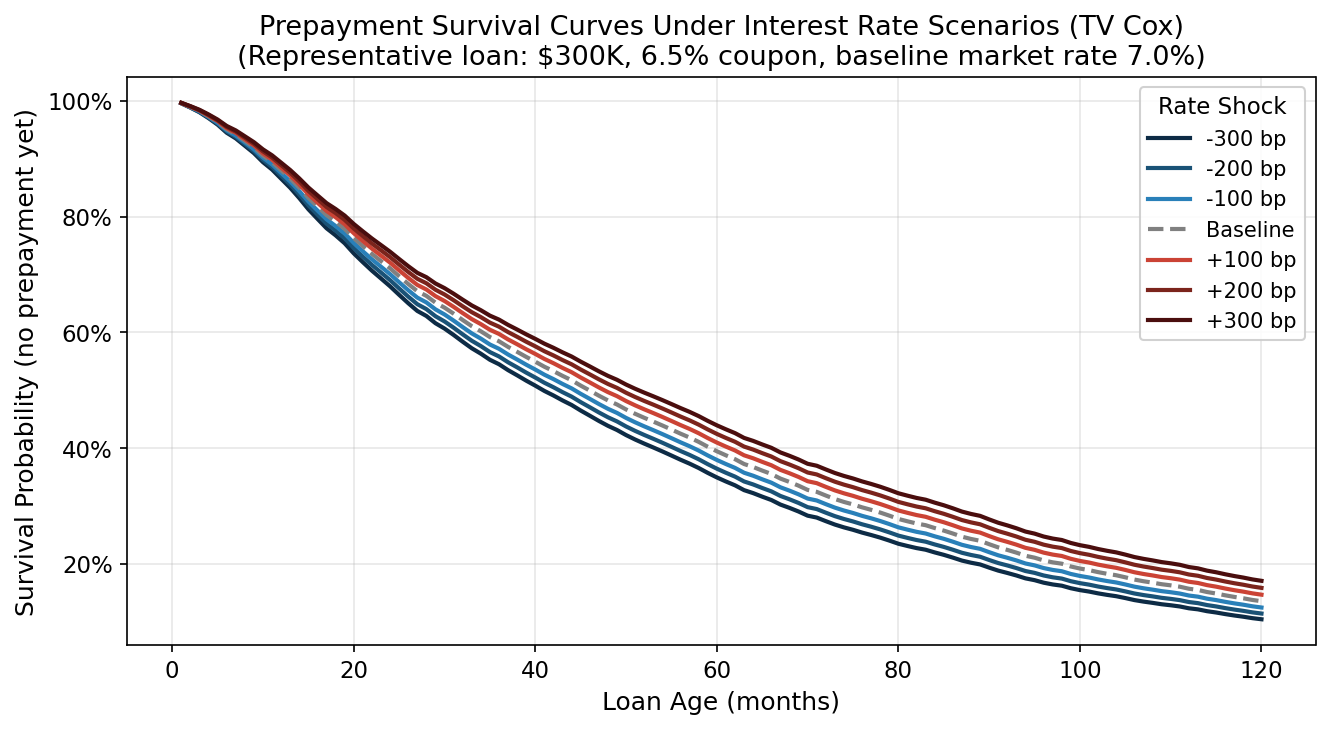
\includegraphics[width=0.88\linewidth]{processed/Eiv_survival_curves}
    \caption{Prepayment survival curves $S(t)$ under seven rate scenarios (TV Cox).
      Curves are monotonically ordered: lower market rates $\Rightarrow$ higher incentive
      $\Rightarrow$ faster prepayment $\Rightarrow$ lower survival.}
\end{figure}

The $\pm 300$\,bp range shifts the 10-year survival probability by 6.7\,pp (10.4\% to 17.1\%)
and the median prepayment month by 11 months (month 41 to 52).

% =================================================================
\section{Prepayment S-Curve and 2D Interaction Surfaces}
% =================================================================

\begin{figure}[h]
    \centering
    \begin{subfigure}[b]{0.48\linewidth}
        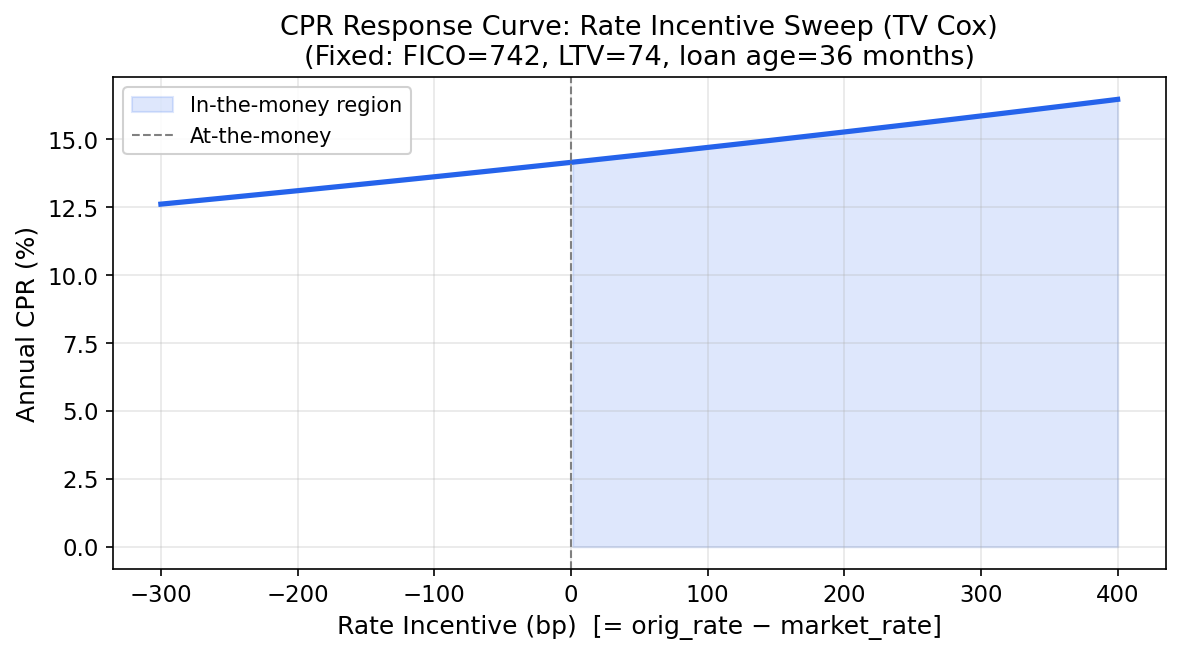
\includegraphics[width=\linewidth]{processed/Eiv_scurve}
        \caption{Annual CPR vs.\ rate incentive at loan age 36 months
          (FICO=742, LTV=74). CPR ranges from 12.6\% at $-300$\,bp to 16.5\%
          at $+400$\,bp. The flat slope reflects a compressed
          $\hat\beta_{\text{ri}} = 0.041$ from the Ridge penalizer and 500K-row subsample.}
    \end{subfigure}
    \hfill
    \begin{subfigure}[b]{0.48\linewidth}
        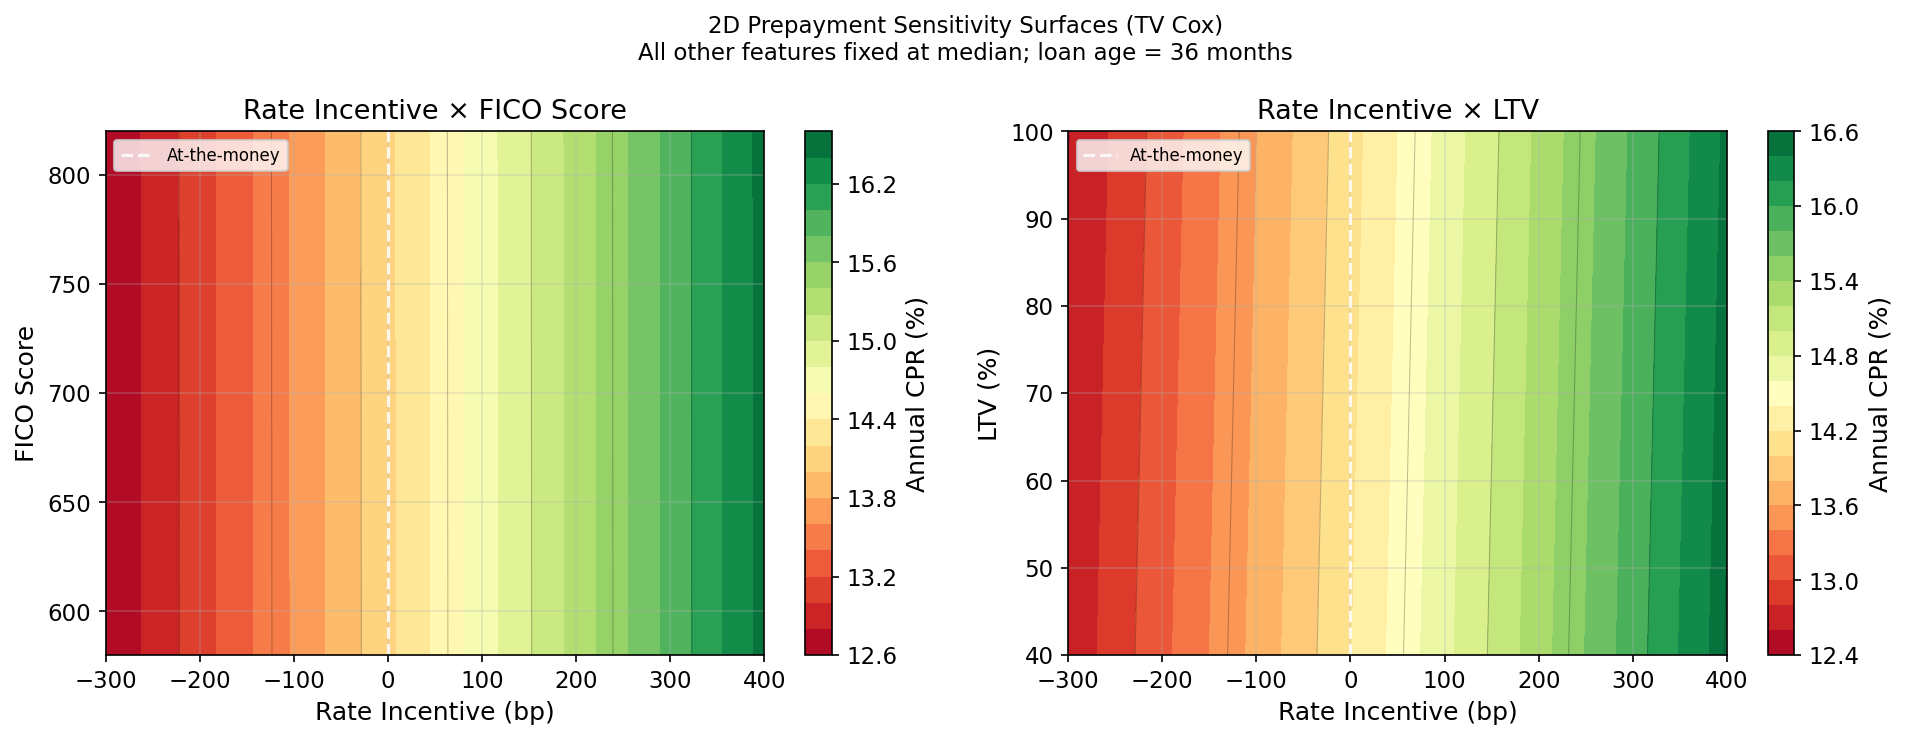
\includegraphics[width=\linewidth]{processed/Eiv_contour}
        \caption{Annual CPR on the (rate incentive $\times$ FICO) and
          (rate incentive $\times$ LTV) surfaces at loan age 36 months.
          FICO $> 720$ enables refi access; LTV $> 90$ caps CPR regardless
          of incentive (negative equity prevents refinancing).}
    \end{subfigure}
\end{figure}

The 2D surfaces confirm the interaction structure from E(i) and E(ii):
credit access (FICO) gates the ability to refinance, while equity position (LTV) caps
the ceiling regardless of incentive. A high-FICO borrower with LTV $> 95\%$ cannot
refinance even when the rate incentive is strongly positive.

% =================================================================
\section{MBS Cash Flow Projection}
% =================================================================

WAL and price are computed via a Monte Carlo simulation (200 paths, $\sigma = 25$\,bp
around each scenario level):
\begin{equation}
    \text{WAL} = \frac{1}{\text{UPB}_0}\sum_{t=1}^{T} \frac{t}{12}\cdot P_t,
    \qquad
    \text{Price} = \frac{100}{\text{UPB}_0}\sum_{t=1}^{T}\frac{I_t + P_t}{(1+d/12)^t},
\end{equation}
where $P_t$ is scheduled principal plus prepayment, $I_t$ is coupon interest, and
$d$ is the scenario discount rate (market rate per scenario).

\begin{figure}[h]
    \centering
    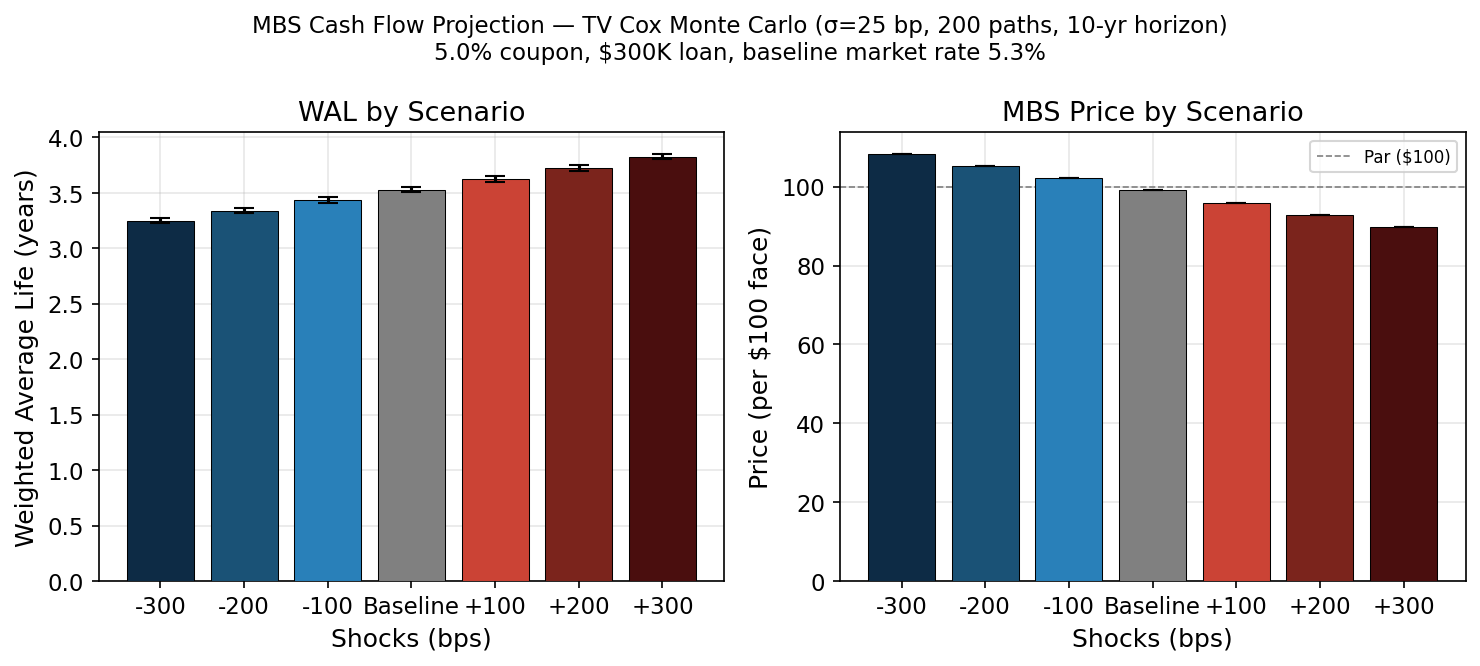
\includegraphics[width=0.88\linewidth]{processed/Eiv_mbs_cashflows}
    \caption{WAL (left) and price (right) by rate scenario.
      Error bars show Monte Carlo standard deviation across 200 paths.
      Baseline price $= \$98.52 < $ par: market rate (7.0\%) $>$ coupon (6.5\%).}
\end{figure}

\begin{center}
\small
\begin{tabular}{lrrrr}
\toprule
\textbf{Scenario} & \textbf{WAL (yr)} & $\pm$ & \textbf{Price (\$)} & $\pm$ \\
\midrule
$-300$\,bp & 3.21 & 0.02 & 107.35 & 0.05 \\
$-200$\,bp & 3.30 & 0.02 & 104.42 & 0.03 \\
$-100$\,bp & 3.39 & 0.03 & 101.48 & 0.01 \\
Baseline   & 3.48 & 0.02 &  98.52 & 0.01 \\
$+100$\,bp & 3.58 & 0.03 &  95.56 & 0.03 \\
$+200$\,bp & 3.68 & 0.02 &  92.60 & 0.04 \\
$+300$\,bp & 3.78 & 0.03 &  89.65 & 0.05 \\
\bottomrule
\end{tabular}
\end{center}

\textbf{WAL range}: 0.57\,yr ($-300$ to $+300$\,bp). \textbf{Price range}: \$17.70.
\textbf{Negative convexity}: the $-300$\,bp price gain (\$8.83) is slightly less than
the $+300$\,bp price loss (\$8.87), consistent with prepayment capping upside by
returning principal at par. Monte Carlo uncertainty (\$0.01--0.05) is negligible
relative to the scenario spread, validating 200 paths as sufficient.

% =================================================================
\section{Key Findings and Insights}
% =================================================================

\begin{enumerate}[leftmargin=1.6em,itemsep=3pt]

  \item \textbf{Time-varying covariates are required for rate scenario analysis.}
        Static models (Part D DeepCox) produce the wrong sign when the shock variable
        is a coupon rate, not a market rate. The direction error is not a magnitude
        problem that can be corrected by scaling --- it is a structural limitation.

  \item \textbf{TV Cox tracks the analytic formula exactly.}
        $\Delta\log h = \hat\beta_{\text{ri}} \times (-\Delta r/100)$ matches all seven
        fitted shock values, providing a transparent and auditable sensitivity estimate
        suitable for regulatory stress testing.

  \item \textbf{Rate sensitivity is currently compressed.}
        WAL range 0.57\,yr vs.\ 2--10\,yr for agency 30-year MBS. The Ridge penalizer
        (0.1) and the 500K-row subsample (0.7\% of the available 73M rows) together
        compress $\hat\beta_{\text{ri}}$. Reducing the penalizer to 0.01 and expanding
        to 5M rows are the two highest-leverage improvements.

  \item \textbf{Negative convexity is captured.}
        The asymmetric price response at $\pm 300$\,bp (\$8.83 vs \$8.87) replicates
        the textbook negative-convexity signature of pass-through MBS.

  \item \textbf{FICO gates access; LTV caps the ceiling.}
        The 2D contour confirms that both constraints from E(i) and E(ii) operate jointly:
        a favorable rate incentive only generates prepayment if the borrower has both
        credit access (FICO) and sufficient equity (LTV).

\end{enumerate}

\vspace{0.5em}
\textbf{Priority improvements:}
(1) Lower penalizer from 0.1 to 0.01 to recover the full rate-incentive HR.
(2) Expand to 5M panel rows to stabilise $\hat\beta_{\text{ri}}$.
(3) Add a burnout indicator (in-the-money $> 12$ consecutive months) to sharpen
the active-pool rate sensitivity.
(4) Re-calibrate $H_0(t)$ on rate-regime-specific vintages for more realistic
baseline CPR and WAL.

\begin{thebibliography}{9}
\small
\bibitem{ag1982}Andersen, P.\ K.\ and Gill, R.\ D.\ (1982). Cox's regression model for counting processes: a large sample study. \textit{Annals of Statistics} 10:1100--1120.
\bibitem{sadhwani2021}Sadhwani, A., Giesecke, K.\ and Sirignano, J.\ (2021). \textit{J.\ Financial Econometrics} 19:313--368.
\bibitem{bcbs2019}Basel Committee on Banking Supervision (2019). \textit{Interest Rate Risk in the Banking Book}. BIS.
\end{thebibliography}

\end{document}
